\section{Monitoring Network Traffic}

\begin{frame}
   {Where Did It Go?}
      \begin{itemize}
	      \item \textbf{ping}
	      \item \textbf{ss}
	      \item \textbf{tracepath}
	      \item \textbf{tcpdump}
	      \item Wireshark
		      
      \end{itemize}


\end{frame}

\cprotect\note{

}


\begin{frame}
	{The \textbf{ss} Command}
      \begin{itemize}
	      \item Dump socket statistics
	      \item Wide range of options and output
      \end{itemize}
	\begin{raw}
$ ss -o state established
$ ss -s
$ ss -a
      \end{raw}


\end{frame}

\cprotect\note{

}


\begin{frame}
   {tracepath}
      \begin{itemize}
	      \item Replacement for \textbf{traceroute}
         \item Doesn't require super-user
	 \item UDP traffic to avoid ICMP issues
      \end{itemize}
	\begin{raw}
$ tracepath linux.com
1?: [LOCALHOST]                      pmtu 1500
1:  gatewaylogin.info                                     3.294ms 
1:  gatewaylogin.info                                     3.068ms 
....
	\end{raw}

\end{frame}

\cprotect\note{

}


\begin{frame}
   {tcpdump}
      \begin{itemize}
         \item Capture all traffic on an interface
	 \item Requires super-user
	 \item Many options and filters
		 \begin{raw}
$ sudo tcpdump -i wlp1s0 -A
tcpdump: verbose output suppressed, use -v or -vv for full protocol decode
listening on wlp1s0, link-type EN10MB (Ethernet), capture size 262144 
01:35:13.439644 ARP, Request who-has 10.71.5.78 tell gatewaylogin.info
..........E.).
G........
G.N..................
01:35:13.442330 IP Txs-Dell.60252 > dns.google.domain: 10558+ PTR? 
78.5.71.10.in-addr.arpa. (41)

		 \end{raw}
      \end{itemize}


\end{frame}

\cprotect\note{

}


\begin{frame}
   {ping}
      \begin{itemize}
         \item Uses ICMP echo response 
	 \item Reports round-trip time
	 \item Often blocked by firewalls
      \end{itemize}
	\begin{raw}
$ ping -c3 linux.com
PING linux.com (151.101.1.5) 56(84) bytes of data.
64 bytes from 151.101.1.5 (151.101.1.5): icmp_seq=1 ttl=252 time=14.5 ms
64 bytes from 151.101.1.5 (151.101.1.5): icmp_seq=2 ttl=252 time=19.2 ms
64 bytes from 151.101.1.5 (151.101.1.5): icmp_seq=3 ttl=252 time=18.0 ms

--- linux.com ping statistics ---
3 packets transmitted, 3 received, 0% packet loss, time 2003ms
rtt min/avg/max/mdev = 14.541/17.300/19.267/2.015 ms
	\end{raw}


\end{frame}

\cprotect\note{

}


\begin{frame}
   {Wireshark}
      \begin{itemize}
         \item Requires super-user to capture all traffic
	 \item Lots of filters
	 \item Dig deep into every packet
      \end{itemize}
      \begin{figure}[H]
         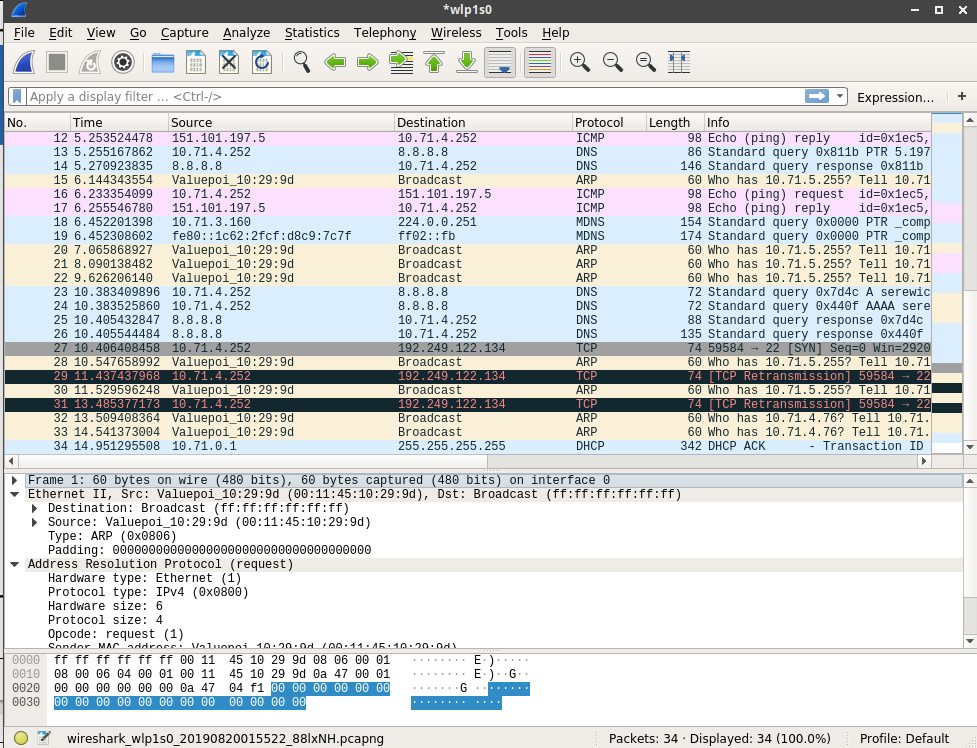
\includegraphics[width=3.4in]{IMAGES/wireshark}
         \caption{Capture Traffice with Wireshark}
      \end{figure}


\end{frame}

\cprotect\note{

}

